\section{Expérimentation}

\subsection{Analyseur statique}

\begin{frame}{L'analyseur \texttt{ptrtype}}

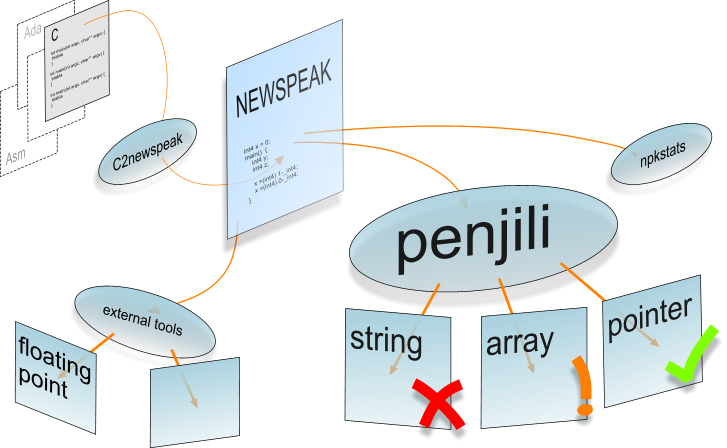
\includegraphics[scale=.5]{img/penjili.png}

\begin{tikzpicture}[remember picture, overlay]

    \node at ($ (current page.north) + (-1.5, -3.7) $) (A) {};
    \node[ draw
         , shape=ellipse
         , shade
         , top color=cyan!30
         , bottom color=white
         , draw=blue!40!black!60
    ] at ($ (A) + (4, 1.5) $) (PT) {\texttt{ptrtype}};

    \node[ draw
         , shade
         , top color=cyan!30
         , bottom color=white
         , draw=blue!40!black!60
    ] at ($ (A) + (1.5, 1) $) (SP) {\scriptsize \langname};

    \node at ($ (PT) + (2.5, 0.5) $) (PTOK) {\parbox{2cm}{\centering Analyse par typage}};

    \draw[thick, orange, ->] (A) to[bend left=10] (SP);
    \draw[thick, orange, ->] (SP) to[bend left=10] (PT);
    \node at ($ (PT) + (-2, 1) $) (ANN) { Annotations };

    \draw[thick, orange, ->] (PT) to[bend left=10] (PTOK);
    \draw[thick, orange, ->] (ANN) to[bend left=10] (PT);
    \path (A) rectangle ++ (7cm, 2cm);

\end{tikzpicture}

\end{frame}

\begin{frame}{Traduction}
\begin{block}{Code C}
\insertcode{tc-c.c}
\end{block}

\only<1>{
\begin{block}{\langname}
\insertcode{tc-ml.c}
\end{block}
}

\only<2>{
\begin{block}{\langname + types inférés}
\insertcode{tc-ty.c}
\end{block}
}

\end{frame}

\subsection{Utilisation sur le noyau Linux}

\begin{frame}[fragile]{Code avec bug}
    % left bottom right top
    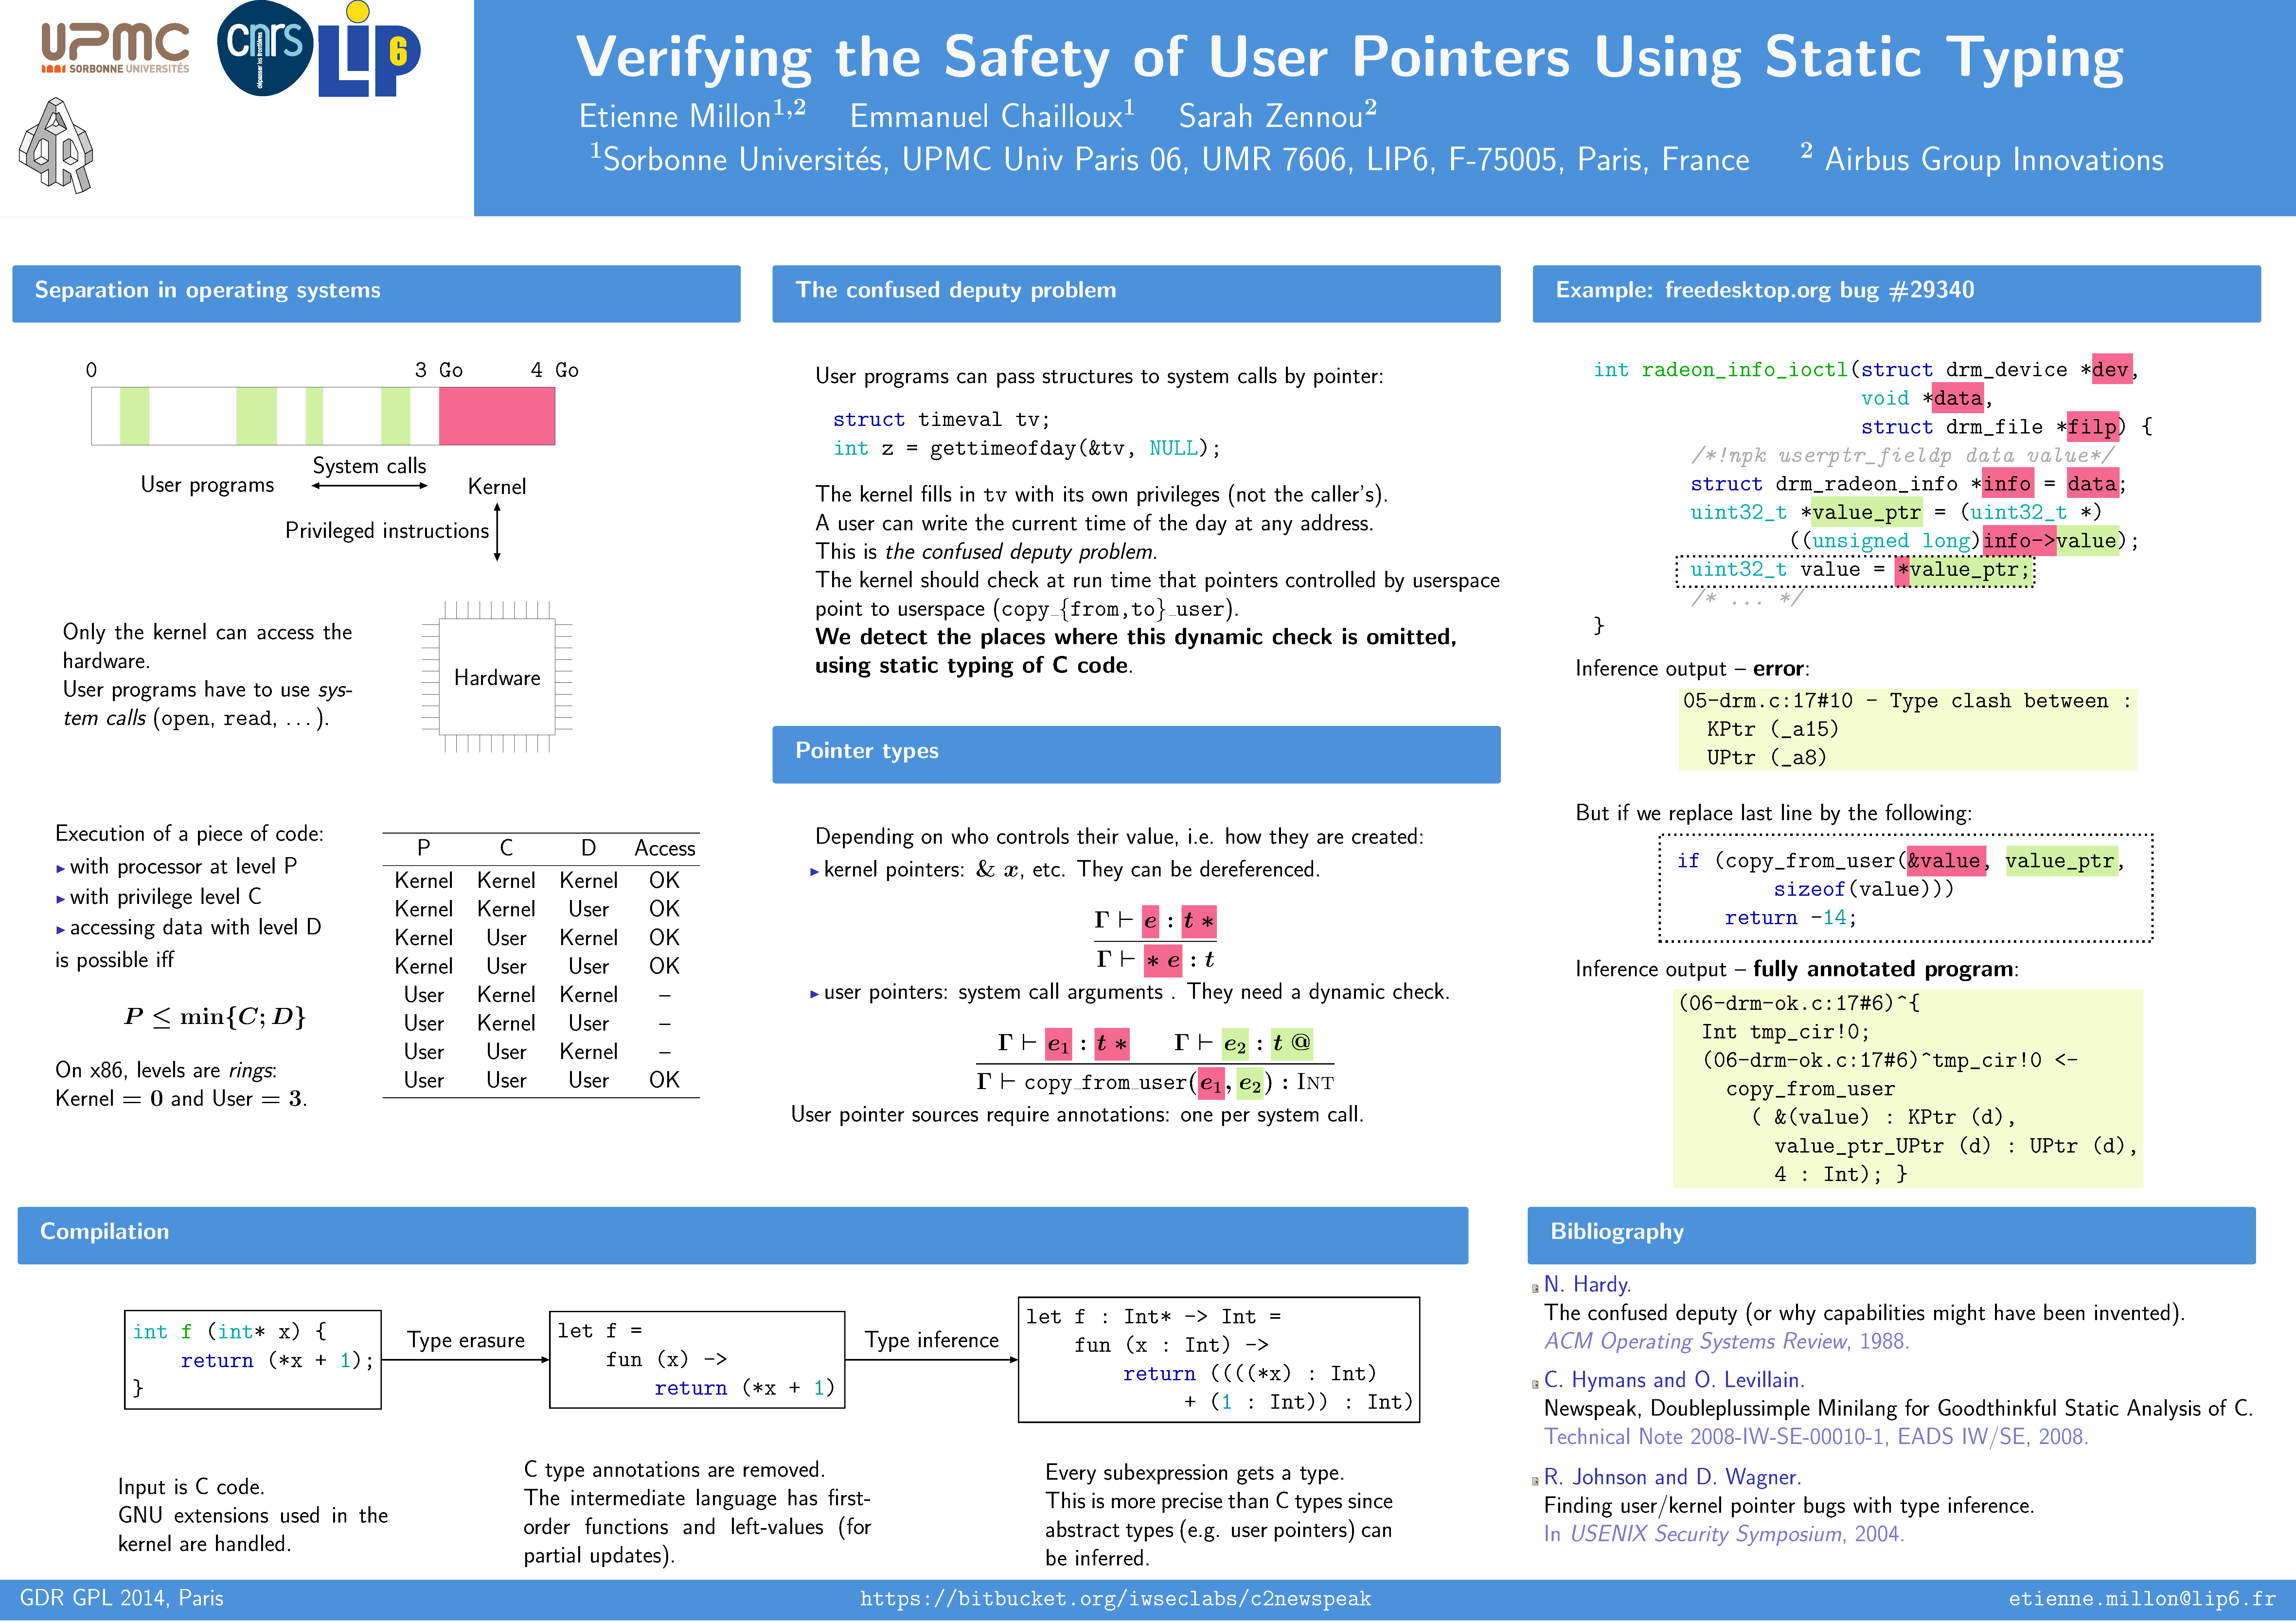
\includegraphics[trim=2300 1430 100 500,clip,width=\textwidth]{poster.pdf}

\begin{SaveVerbatim}{drmko}
05-drm.c:17#10 - Type clash between :
  KPtr (_a15)
  UPtr (_a8)
\end{SaveVerbatim}

% TODO impact de ce bug?

\codeout{drmko}
% ne pas parler des inconnues
\end{frame}

\begin{frame}[fragile]{Code corrigé}
    % left bottom right top
    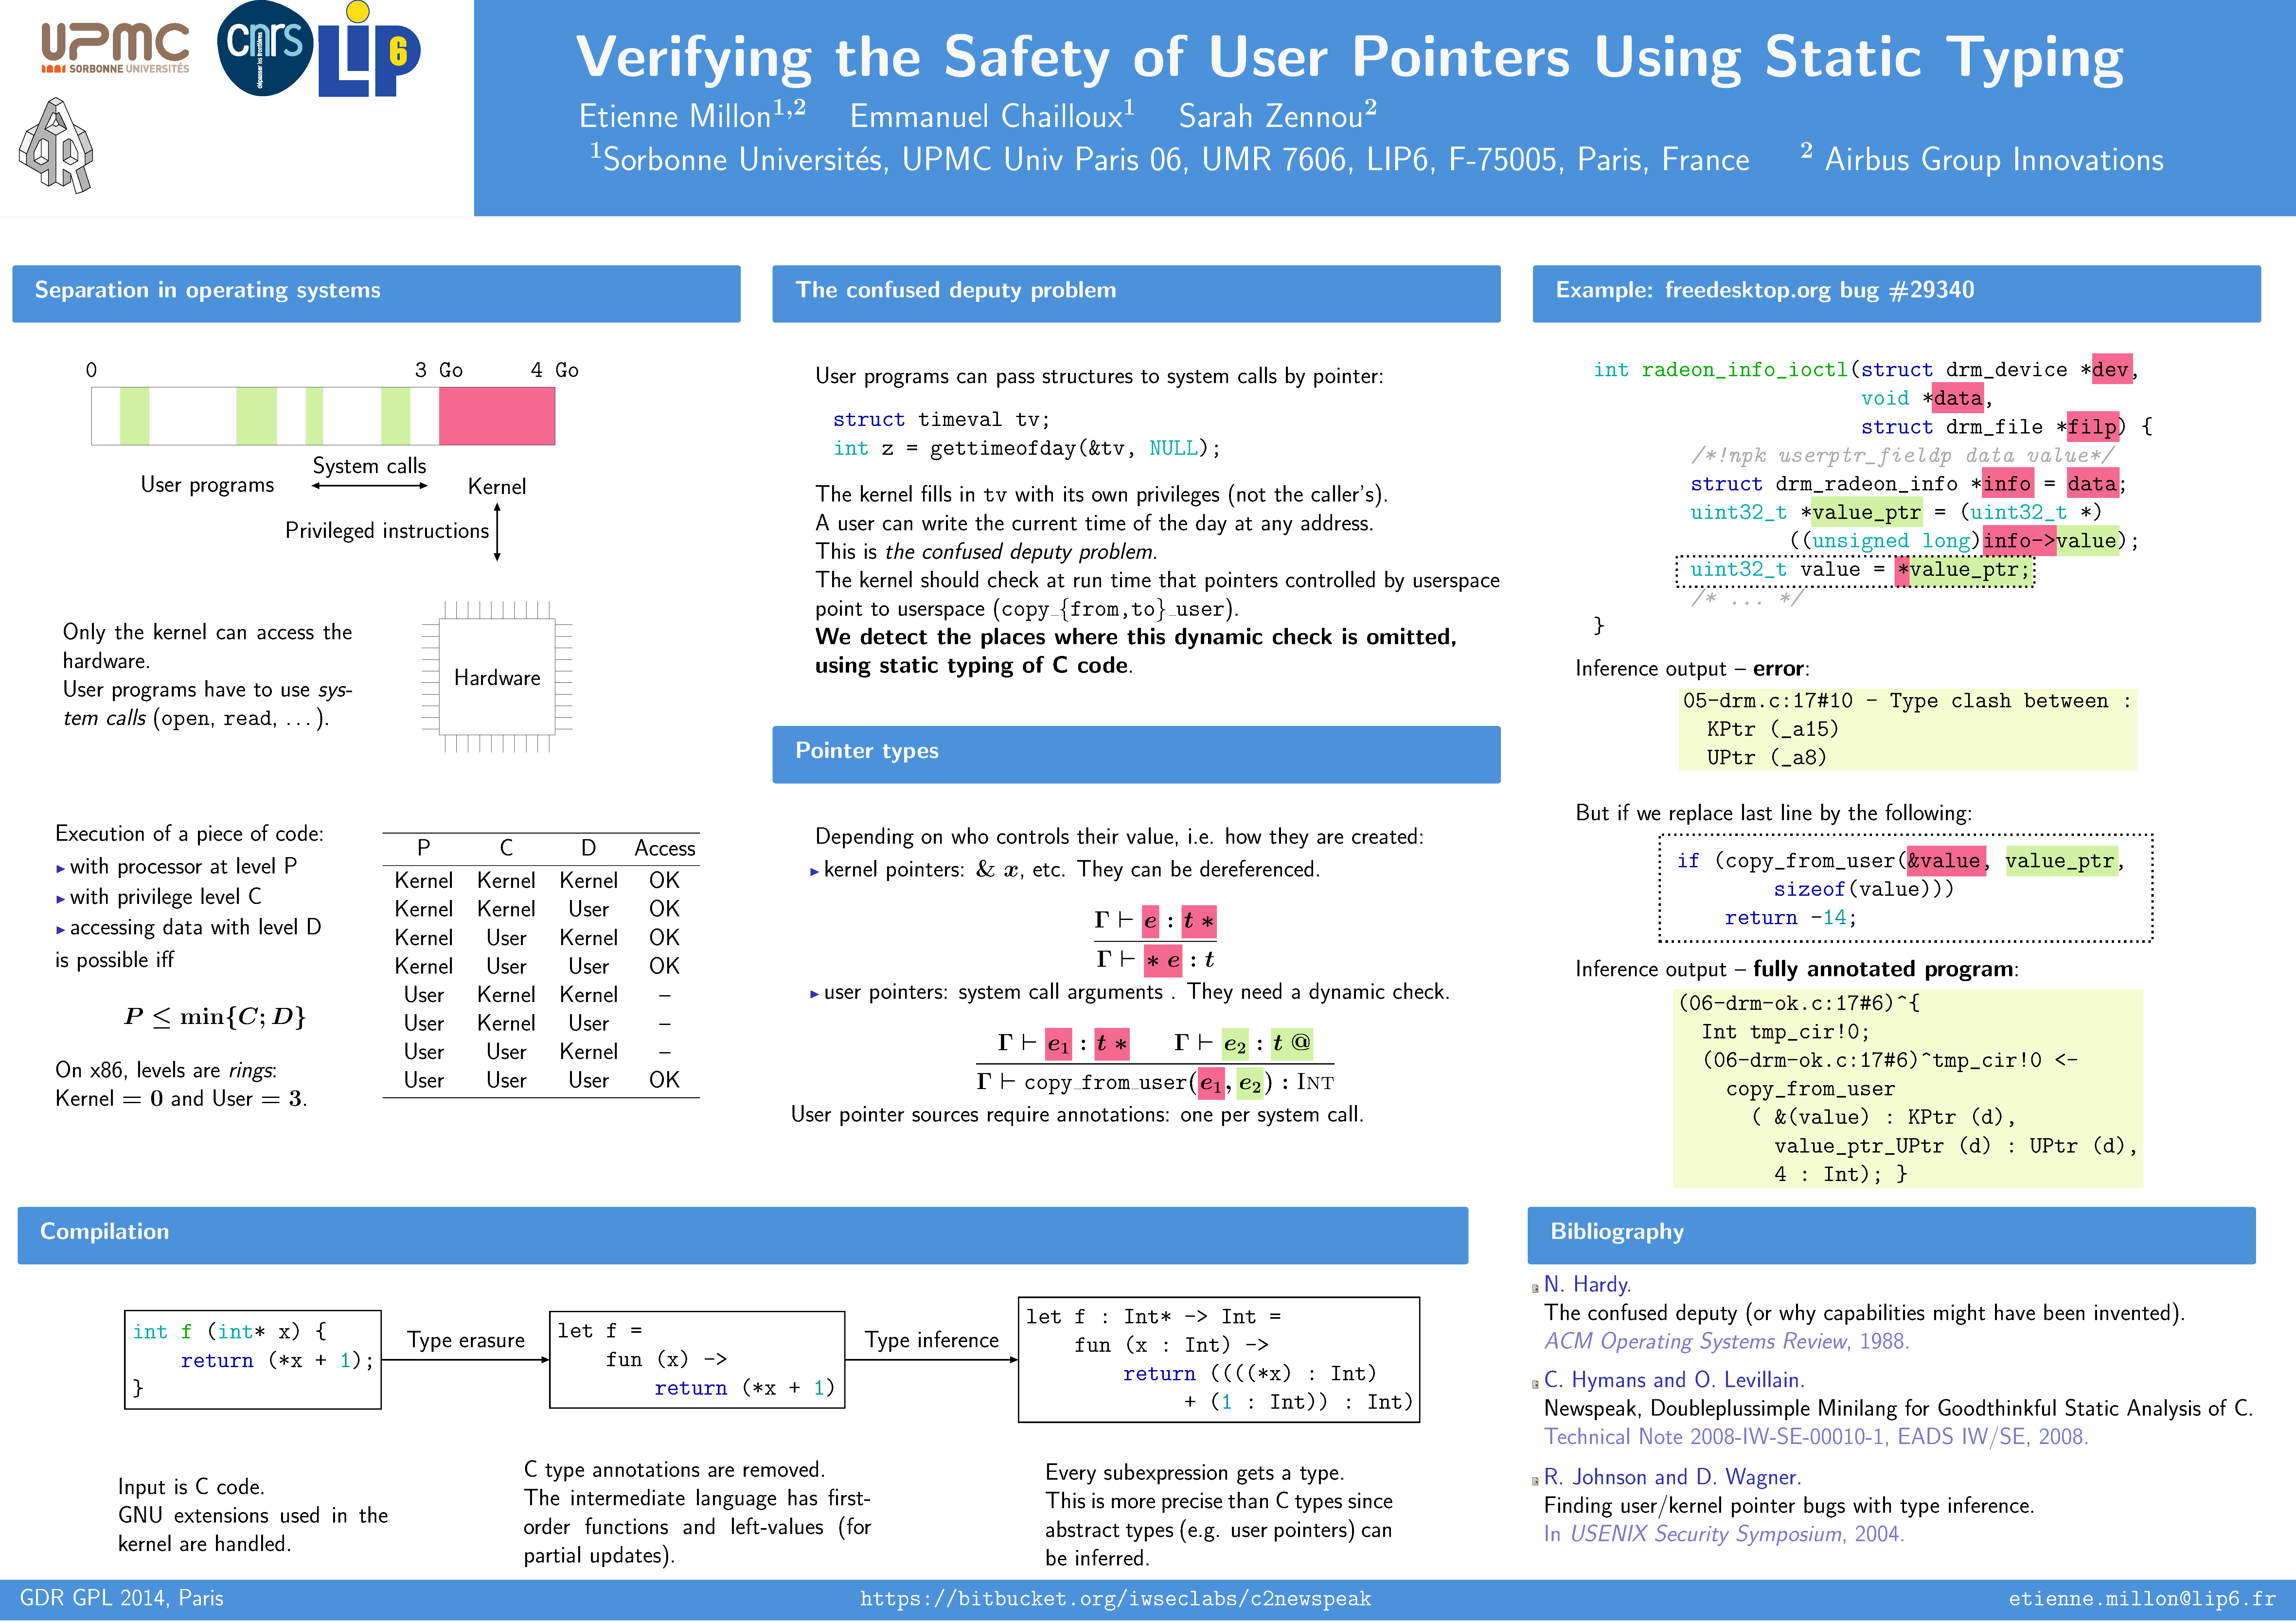
\includegraphics[trim=2300 990 100 1220,clip,width=\textwidth]{poster.pdf}

\begin{SaveVerbatim}{drmok}
(06-drm-ok.c:17#6)^{
  Int tmp_cir!0;
  (06-drm-ok.c:17#6)^tmp_cir!0 <-
    copy_from_user
      ( &(value) : KPtr (d),
        value_ptr_UPtr (d) : UPtr (d),
        4 : Int); }
\end{SaveVerbatim}

\codeout{drmok}
\end{frame}
